\documentclass{article}

\usepackage[utf8]{inputenc}
\usepackage[T1]{fontenc}      
\usepackage[francais]{babel}
\usepackage{graphicx}
\usepackage{circuitikz}
\usepackage[squaren, Gray]{SIunits}
\usepackage{sistyle}
\usepackage[autolanguage]{numprint}
\usepackage{pgfplots}
\pgfplotsset{compat=1.9}
\usepackage{amsmath,amssymb,array}
\usepackage[top=2.5cm,bottom=2.5cm,right=2.5cm,left=2.5cm]{geometry}
\usepackage{url} 
\usepackage{tabularx}
\DeclareMathOperator{\dist}{d}
\newenvironment{abstract-fr}
{
	\begin{center}
		\textbf{Résumé} \\[0.5cm]
	\end{center}
}
{}

\newenvironment{abstract-en}
{
	\begin{center}
		\textbf{Summary} \\[0.5cm]
	\end{center}
}
{}
% New command pour la modélisation mécanique, tri à effectuer
\newcommand\fv[1]{{\bf #1}} % free vector
\newcommand\fvd[1]{\dot{\bf #1}} % free vector derivated
\newcommand\fvdd[1]{\ddot{\bf #1}} % free vector derivated
\newcommand\fvr[1]{\mathring{\bf #1}} % free vector relatively derivated
\newcommand\fvrr[1]{\overset{\circ\circ}{\bf #1}} % free vector relatively derivated
\newcommand\uv[1]{{\bf\hat{ #1}}} % unit vector
\newcommand\ui{{\bf\hat{I}}} % unit vector I
\newcommand\uj{{\bf\hat{J}}} % unit vector J
\newcommand\uk{{\bf\hat{K}}} % unit vector K
\newcommand\wrt[2]{\ensuremath{\tensor*[_{ #1}]{ #2}{}}} % With Respect To
\newcommand\wtr[3]{\ensuremath{\tensor*[_{ #1}]{ #2}{^{ #3}}}} % With Two Respect
\newcommand\omegaf{{\bm \omega}}
\newcommand\omegafr{\mathring{\bm \omega}}
\newcommand\omegafd{\dot{\bm \omega}}
\newcommand\omegaft{\tilde{\bm \omega}}
\newcommand\omegaftr{\mathring{\tilde{\bm \omega}}}
\newcommand\omegat{\tilde{\omega}}
\newcommand\omegatd{\tilde{\dot{\omega}}}
\newcommand\ine{{\bf I}}
\newcommand\st{{\bf L}}
\newcommand\pst{{\bf M}}
\newcommand\lm{{\bf N}}
\newcommand\am{{\bf H}}
\newcommand\amd{\dot{\am}}
\newcommand\fo{{\bf F}}
\newcommand\po{\mathcal{P}}
\newcommand\xg{\ensuremath{\fv{R}}}
\newcommand\xgd{\ensuremath{\fvd{R}}}
\newcommand\xgdd{\ensuremath{\fvdd{R}}}
\newcommand\dvec[1]{\dot{\vec{ #1}}}
\newcommand\ddvec[1]{\ddot{\vec{ #1}}}
\newcommand\qp{\dot{q}}
\newcommand\dqp{\Delta \dot{q}}
\usepackage{url} 
\usepackage{hyperref}
\hypersetup{
    colorlinks,
    citecolor=black,
    filecolor=black,
    linkcolor=black,
    urlcolor=black
}

\begin{document}

% L'objectif du projet + les spécifications attendues + cahier des charges (ref)
Dans le cadre du cours \textit{Projet 2} du deuxième quadrimestre, notre groupe a été amené à 
concevoir un haut-parleur connectable, via une prise Jack \unit{3.5}{\milli\meter}, à un 
GSM ou un MP3 (les contraintes et spécifications sont détaillées dans l'annexe ''Cahier des charges''). 
En plus de cela, notre haut-parleur doit permette un règlage du volume, des graves
et des aigus. Un autre objectif du projet est d'apprendre un travailler et à s'organiser \textit{en groupe}, 
comme le font tous les jours les ingénieurs.

% L'organisation du rapport
Ce rapport s'articule principalement en deux grands chapitres. Le premier
rassemble les différentes étapes de modélisations mathématiques
et physiques de composants du haut-parleur. Dans ce chapitre, nous 
commencerons par une vue générale du haut-parleur qui nous
permettra d'introduire les concepts physiques clés. Nous continuerons
ensuite par la modélisation des filtres passe-bas, passe-haut et passe bande.
Après cela, nous nous attarderons  sur le dimensionnement de l'électroaimant et
de la bobine mobile pour enfin terminer par la modélisation mécanique de la bobine
mobile.

Le deuxième chapitre contient quant à lui la synthèse des recherches documentaires
effectuées. Ces recherches portent sur deux sujets liés à notre haut-parleur. Le premier
concerne plutôt l'acoustique, il s'agit de la 
distorsion harmonique. Le deuxième quant à lui concerne un concept lié au circuit électrique qui
compose notre haut-parleur, il s'agit du principe de la contre-réaction.

% Description générale du système
Penchons-nous sans plus tarder sur une description générale du système. Notre haut-parleur
peut-être représenté schématiquement comme sur la Figure \ref{block-diagram-hp}.

% Schéma montrant le bonne compréhension du système
\begin{figure}[!htb]
	\centering
	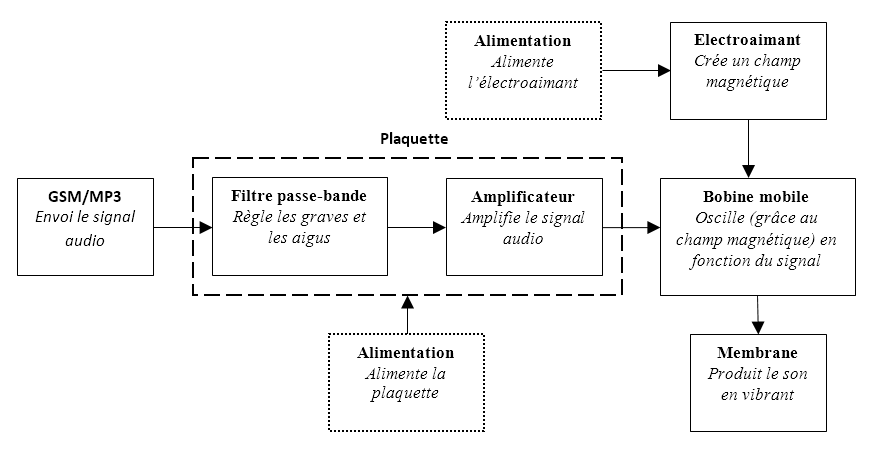
\includegraphics[scale=0.68]{schema_fonctionnel.png}
	\caption{Schéma fonctionnel du haut-parleur.}
	\label{block-diagram-hp}
\end{figure}

Le GSM ou le MP3 va dans un premier temps envoyé un signal audio via le cable Jack au circuit
imprimé, par la suite nous qualifierons ce signal de \textit{brute}. Le circuit imprimé permet
quant à lui de modifier ce signal brute de plusieurs façon : 

\begin{itemize}
	\item En règlant le volume, c'est à dire en modifiant l'amplitude du signal audio ;
	\item En règlant les graves et les aigus, c'est à dire en atténuant les basses ou les hautes
	fréquences. Il s'agit du rôle des filtres passe-bas et passe-haut qui combiné forme un filtre 
	passe-bande ;
	\item En amplifiant le signal : c'est le rôle de l'amplifcateur audio du circuit.
\end{itemize}

A la sortie du circuit imprimé, le signal est alors \textit{filtré} et \textit{amplifié}.
Ce signal traité ira ensuite alimenter en courant la bobine mobile. Cette 
dernière intercepte un champ magnétique constant, noté $B$, produit par l'électroaimant.
Elle subit donc une force de \textsc{Laplace} dont l'expression est :

$$\vec{F} = i(t)\vec{L}\times{\vec{B}}$$ 

Où $L$ est la longueur du fil et$i(t)$ le courant le traversant. Cette force est proportionnelle
au courant traversant
la bobine mobile. La membrane se déplacera donc de manière cohérente avec le signal audio
et reproduira le son voulu. Enfin, la membrane pourra revenir à son position d'équilibre
grâce à des attaches qui, à la manière de ressorts, produisent une force de rappel.

% Just here to fix rapport_prejury.tex
\end{document}